% This is samplepaper.tex, a sample chapter demonstrating the
% LLNCS macro package for Springer Computer Science proceedings;
% Version 2.20 of 2017/10/04
%
\documentclass[runningheads]{llncs}
%
\usepackage{graphicx}
\usepackage{hyperref}
\renewcommand\UrlFont{\color{blue}\rmfamily}
\setlength{\parskip}{0pt}
\raggedbottom

\usepackage{amsmath}
\usepackage{csquotes}
\usepackage{paralist}
\usepackage{booktabs}
\usepackage{mathptmx}
\usepackage{pgfplots}
\pgfplotsset{compat=1.8}

\begin{document}
%
\title{Towards an efficient Prediction Model\\ of Malaria Cases in Senegal}
%
%\titlerunning{Abbreviated paper title}
% If the paper title is too long for the running head, you can set
% an abbreviated paper title here
%
\author{Ousseynou Mbaye \and Mouhamadou Lamine Ba \\ Gaoussou Camara \and Alassane Sy}
%
\authorrunning{Ousseynou Mbaye \and M. Lamine Ba \and Gaoussou Camara \and Alassane Sy}
% First names are abbreviated in the running head.
% If there are more than two authors, 'et al.' is used.
%
\institute{Universit\'e Alioune Diop de Bambey, Bambey, Senegal\\
\email{firstmidlle.last@uadb.edu.sn}
%\email{ousseynou.mbaye@uadb.edu.sn}\\
%\email{mouhamadoulamine.ba@uadb.edu.sn}\\
%\email{gaoussou.camara@uadb.edu.sn}\\
%\email{alassane.sy@uadb.edu.sn}
}
%
\maketitle              % typeset the header of the contribution
%
\begin{abstract}
Among  the most deadly disease in the world, Malaria remains a real flail in Sub-saharan Africa 
in particular. In countries like Senegal, such a situation is acute due to the lack of high quality
healthcare services and well-formed staffs able to perform accurate diagnosis of diseases that patients suffer from. 
This calls for the need of finding automated tools to help medical actors in their decision making process.
In this paper, we present first steps towards an efficient way to automatically diagnosis Malaria occurence or not 
based on patient signs and symptoms, and the outcome from the quick diagnosis test. Our prediction approach is built
on the logistic regression function. First expermients on a real world patient dataset, as well as a semi-synthetic dataset,
show promising performance results regarding the effectiveness of the proposed approach.
 
\keywords{Malaria  \and Diagnosis \and Data imputation \and Prediction Model.}
\end{abstract}
%
%
% Introduction
\section{Introduction}\label{intro}











% Papier organization

The remaining of the paper is organized as follows. We summarize the related work on data imputation and binary classification methods in Section \ref{related_work}.
In Section \ref{data_prep} we introduce the data profiling and imputation techniques used on patient records. We then present our prediction model for Malaria cases in Section \ref{prediction_model}.
Experimentation on real-world datasets are detailled in Section \ref{experimentation} before we conclude in Section \ref{conclusion}. 


% Related work
\section{Related work}\label{related_work}
In this section, we summarize the sate-of-the-art research on Malaria in general, and in particular the
use of machine learning techniques to tackle the various aspects related to one of the 
major healthcare problems worldwide which is Malaria.

% Studies on Malaria
As it is well-known, Malaria is caused by the bite of the female Anopheles, the most dangerous of which
is Plasmodium falciparum. Many early works have been consequently focused on the study of the evolution and
the distribution of the responsible mosquito, mainly with the goal to detect or diagnosis the severity of the 
disease given an infected patient \cite{Fe03,Al09}. Recent research on Malaria have largely adopted machine learning
and showed its ability to solve various aspects of the disease. Most of these machine learning based techniques are 
based on the analysis of blood data obtained from high-definition microscopic screenshots as in \cite{Ku18}. The authors
in \cite{Ku18} propose an unsupervised learning algorithm that detects and determines the types of infected blood cells.
Used prediction approach consists of quantifying the amount of plasmodium parasites in a blood smear. In the same research intuition
of harnessing blood, the Jordan-Elman neural network classifier introduced in \cite{Ha15}, on the other hand, to quickly determine the occurrence 
of Malaria and its severity level as well: the neural network analyzes the features of the blood data of the patients.  
Still using ML, DIAZ et al. have proposed in \cite{Dia09} a semi-supervised algorithm enable to quantify and classify the 
erythrocytes infected by Malaria parasistes through microscopic images. The orginiality of this work comes from its usability
even in the presence of thin blood drandruff infected by falciparum Plasmodium for the quantification and the classificationi tasks.
Besides blood data, sign and symptom records were also used to study Malaria with ML methods. Indeed, decision trees based approach
has been proposed in Nigeria \cite{Ug10} to predict the occurrence of Malaria given diagnostic data. However a decision tree suffers 
from various limitations as a classifier. Indeed it can easily overfit or can be extremely sensitive to small pertubations in data for instance.
Even though we both rely on signs and symptoms, the prediction model in \cite{Ug10} differs from ours on numerous facets: our model is built upon
logistic regression and is trained using also inputs from the quick diagnosis test. In addition, we apply our method in the context of patients living in Senegal. 



% Data Preparation
\section{Data imputation}\label{data_prep}
\subsection{Description des données}
Le jeu de données alldataoriginalcopie
comporte 21083 patients et 16 attributs. Les attributs sont entre autres les données nominatives des patients, les signes et les symptômes constatés par le médecin, le traitement proposé, le diagnostic  final du médecin, les résultats du TDR (Test de Diagnostic Rapide)  et le statut (hospitalisation, décès ou mis en observation) du patient.
Insérer tableau ici
On remarque que les attributs tels que signeSymptome et  Diagnostic sont multivariés. Ainsi nous devrons les splitter pour récupérer les informations qui sont pertinentes pour notre étude à savoir prédire si un patient présentant un certain nombre de signes et symptômes est atteint de paludisme ou non
\subsection{Sélection  des signes et symptômes   du paludisme}
Toutes les informations contenues dans la colonne signeSymptome ne sont pas utiles pour diagnostiquer un  paludisme. Ainsi pour notre étude nous avons extrait 12 nouveaux attributs qui sont les signes et les symptômes du paludisme. Ces attributs sont les suivants : manque d'appétit, fatigue, arthralgie, trouble digestif, vertiges, frisson, myalgie, diarrhée et  douleur abdominale.
Le Diagnostic est le résultat des signes et symptômes confirmé par un examen médical en général. 
Dans la colonne Diagnostic, on voit plusieurs conclusions différentes. Ainsi tout diagnostic autre que le paludisme est remplacé par la classe non paludisme. Ainsi la colonne Diagnostic reste multivariée avec les catégories suivantes: accès palustre, paludisme, simple paludisme, paludisme grave, accès paludisme grave, accès paludisme simple, syndrome palustre, paludisme suspect et pas de paludisme ( se sont tous les diagnostics différents du paludisme).
Insérer tableau ici
\subsection{Imputation des données manquantes}
La plus part des attributs de notre jeu de données présente des valeurs manquantes. Ces valeurs manquantes peuvent avoir un impact négatif sur notre analyse future. Pour remplacer ces dernières, nous avons utilisé le package missForest du logiciel R.
Pour cela les attributs textuels comme les signes et symptômes ou les classes de l’attribut Diagnostic 
ont été remplacés par des valeurs numériques.
 Avec un  NRMSE de 0,01  nous pouvons dire que l’imputation a réussi mais aussi n’a pas altéré 
 la structure des données.


% Prediction Model
\section{Prediction Model}\label{prediction_model}
To learn from labelled patient dataset and be able to properly predict 
the occurence or not of Malaria given a new patient, we harness the logistic 
regression function as our \emph{classifier}. 
In this section, we briefy recall the basic of the logistic regression function
and how it can act as a binary classifier. We start by introducing the binary 
classification problem we have to solve in the study.

% binary classification problem for Malaria
\subsection{Binary classification problem}
Let us assume two given classes of Malaria diagnostic: \emph{Malaria} and \emph{Not-Malaria}.
We also consider \textsc{P} and \textsc{C} as respectively the set of patients and a prediction model.
A patient \emph{p} in \textsc{P} is defined by a set of pairs $(a_1, v_1), (a_2, v_2), \ldots, (a_n, v_n)$
where $a_i$ and $v_i$, for each $1\leq i\leq n$, respectively corresponds to a given Malaria feature and its associated value defined
as follows.
\begin{equation}
v_i = \left\{
\begin{array}{rl}
1 &\text{if $a_i$ is observed} \\
0 &\text{otherwise} \\
\end{array}
\right.
\end{equation}

\begin{definition}{(Our prediction problem)}
We define our binary classification problem for the prediction of the occurrence
or not of Malaria on a given patient dataset as a mapping \textsc{C} of every patient p in \textsc{P} 
to one and only one class in \{Malaria, Not-Malaria\}. Formally, we present such a mapping as \textsc{C}: \textsc{P} $\mapsto$ \{Malaria, Not-Malaria\}.
\end{definition}


We define and use  \textsc{C} with the help of the logistic regression for the specific purpose of our study. 
% Logistic regession function
\subsection{Logistic regression}
The logistic regression (a.k.a the logit function) is a statistical model used in the machine learning domain for binary classification.
In its basic form, it is based on a logistic function to model a binary dependent variable \cite{Sa14}.
As an input, the logistic regression  takes qualitative or/and ordinal predictive variables (e.g. the presence
or not of fever given a patient) in order to measure the probability of the outcome (e.g. the occurrence or not of the Malaria) 
by using the \emph{Sigmoid function}. Figure \ref{sigmoid_curve} shows the shape of the curve of the Sigmoid function. 

% The curve of the logistic regression
\begin{figure}[ht]
\centering
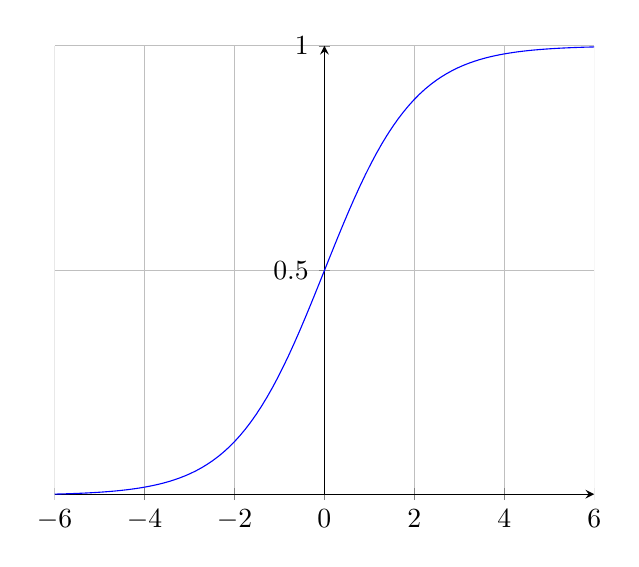
\begin{tikzpicture}
    \begin{axis}%
    [
        grid=major,     
        xmin=-6,
        xmax=6,
        axis x line=bottom,
        ytick={0,.5,1},
        ymax=1,
        axis y line=middle,
    ]
        \addplot%
        [
            blue,%
            mark=none,
            samples=100,
            domain=-6:6,
        ]
        (x,{1/(1+exp(-x))});
    \end{axis}
\end{tikzpicture}
\caption{The curve of the Sigmoid function}\label{sigmoid_curve}
\end{figure}


% Experimentation and Results
\section{Experimentation and results}\label{experimentation}
In this section, we present the performance of our prediction
 model for Malaria occurrecne through an analysis of the results
 of the experimentations we have conducted on real-world datasets
and a semi-synthetic dataset. We start by presenting our experimentation setting.
 
% Experimentation setting
\subsection{Experimentation setting}
We ran tests on three different datasets using the Python Implementation of the logistic regression function.
To impute missing data, we have used the R package of the algorithm missForest.

% Our datasets
\subsubsection{Our datasets.}
We collected and used a real-world patient dataset from the different health points which were set during the Grand Magal of Touba in 2016.
We also generated and used two variants of this real-world dataset. The description of the characteristics of our raw real-world dataset, as well as the  data preparation
pipeline that we have proposed in order to clean, normalize and impute information, are given in Section \ref{data_prep}; we refer to this cleaned and complete real-world
patient dataset by \textsc{DT1}. 

We generated the first variant, denoted by \textsc{DT2}, of the raw real-world patient dataset by 
removing records with missing attributes, instead of using an imputation algorithm that will predicts 
values for missing information. Such a variant will help to study the impact of removing records with 
missing values in the prediction accuracy.
 
The second variant, called \textsc{DT3}, is a semi-synthetic dataset which has been set up by using a 
sampling strategy over our raw real-world dataset. Indeed when we have performed some explanatory analysis 
on the real-world dataset have been revealed that the dataset was not balanced, i.e. it shows strong between
class imbalance; the amount of records about patients suffering from Malaria was largely less than the number
of patients that do not suffer from Malaria as shown in Figure \ref{records_class}. Harnessing sampling approaches may enbale to obtain a balanced 
semi-dataset regarding the two classes to predict. To solve our problem of imbalanced dataset, we used the 
algorithm SMOTE \cite{Wa06}, which is a synthetic minority oversampling technique, through its Python implementation
in the  package \emph{imbalanced-learn} \cite{Gu17}. SMOTE consists of predicting a sample of synthetic dataset based on 
the value of the minority class of the targeted class (here the attribute Diagnostic). It randomly chooses the k-nearest 
neighbours of a given record in order to randomly create new observations.
 We have applied an over-sampling of the minority class into our patient 
dataset for generating  a semi-synthetic dataset \textsc{DT3} containing the same number of records for both classes.  

% distribution of records by class
\begin{figure}[h]
\centering
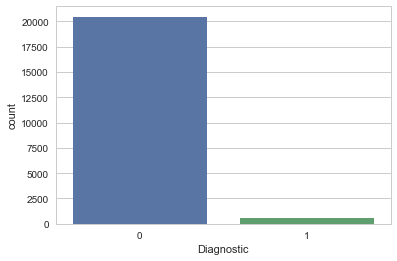
\includegraphics[width=0.6\textwidth]{images/imbalanced_dataset}
\label{records_class}\caption{The number of records by class}
\end{figure} 

% Implementation of the logistic model
\subsubsection{Prediction model setting.}
In order to set up our logistic regression-based classification model, we rely on the Python implementation of the logistic regression in the \emph{sklearn} library\footnote{https://scikit-learn.org/stable/modules/generated/sklearn.linear\_model.LogisticRegression.html}.
This python package defines the logistic regression with the required input parameters, as well as optimization strategies, to properly perform binary 
classification using the best final model. For the purposes of our tests, we have used the following input parameters of the logistic regression:

% input parameters
\begin{itemize}
\item \textbf{random\_state}:
\item \textbf{class\_weight}:
\item \textbf{dual}:
\item \textbf{intercept\_scaling}:
\item \textbf{max\_iter}:
\item \textbf{multi\_class}:
\item \textbf{n\_jobs}:
\item \textbf{penalty}:
\item \textbf{solver}:
\item \textbf{tol:}
\item \textbf{verbose}:
\item \textbf{warm\_start}:
\end{itemize}

As the logistic regression performs a supervised learning we have used 60\% for the training set and 30\% for the test set.

% Performance measures
\subsection{Performance measures}
In medecine, \emph{sensitivity} and \emph{specificity} are often used, 
while in information retrieval \emph{precision} and \emph{recall} are preferred.
An important distinction is between metrics that are independent on the prevalence
(how often each category occurs in the population), and metrics that depend on the
prevalence – both types are useful, but they have very different properties.

% Analysis of the results
\subsection{Experiments and analysis of the results}


\subsubsection{Experiments with DT\_1}
\subsubsection{Experiments with DT\_2}
\subsubsection{Experiments with DT\_3}
\subsubsection{Comparative analysis of the results}


% Conclusion
\section{Conclusion}


%
% ---- Bibliography ----
%
% BibTeX users should specify bibliography style 'splncs04'.
% References will then be sorted and formatted in the correct style.
%
\bibliographystyle{splncs04}
\bibliography{biblio}
%
\end{document}
